% ============================================================
%  CAPÍTULO 4 – RESULTADOS
% ============================================================
Este capítulo presenta los resultados obtenidos por el sistema CAIQ, organizados en torno a los cinco objetivos específicos planteados en la Sección 1.4 (``Objetivos específicos''): (1) descarga y preprocesamiento de datos, (2) actualización y definición continua, (3) desarrollo y comparación de modelos de recomendación, (4) validación cuantitativa y sobre casos de uso, y (5) implementación de la interfaz web. Para cada objetivo se presentan los resultados cuantitativos y cualitativos obtenidos y se valora en qué medida el objetivo correspondiente queda cubierto. La descripción detallada de los métodos, algoritmos y procedimientos que producen estos resultados se encuentra en la Sección~\ref{subsec:arquitectura_general_del_sistema} y siguientes; la interpretación crítica conjunta de estos resultados, sus limitaciones y sus implicaciones se desarrolla en el capítulo de Discusión.

% -----------------------------------------------------------
\subsection{Resultados frente al objetivo 1: descarga y preprocesamiento de datos}
\label{subsec:resultados_obj1}
% -----------------------------------------------------------
El primer objetivo específico exigía construir y preprocesar \textit{datasets} representativos de másteres, cursos y ofertas de empleo, incluyendo su limpieza, normalización y enriquecimiento mediante un \textit{pipeline} ETL.

El sistema dispone de tres \textit{datasets} estructurados y enriquecidos, resumidos en la Tabla~\ref{tab:resumen_datasets}: 37.829 ofertas de empleo limpias y deduplicadas, 89.332 cursos \textit{online} y 3.503 programas de máster, de los cuales 96 se ubican en España. El proceso ETL descrito en la Sección~\ref{subsec:proceso_etl} transforma los registros heterogéneos de la Tabla~\ref{tab:tabla3_1} en el esquema normalizado de la Tabla~\ref{tab:tabla3_2}, generando variables derivadas (\texttt{role\_family}, \texttt{seniority}, \texttt{work\_mode}, \texttt{employment\_type}) y un total de 134.056 pares oferta--competencia mapeados sobre la taxonomía controlada. El detalle del impacto cuantitativo del proceso ETL se presenta en la Sección~\ref{subsec:resultados_obj2}, junto con los resultados del \textit{pipeline} de \textit{scraping}.

\begin{table}[H]
  \caption{Resumen de los \textit{datasets} construidos frente al objetivo 1.}
  \label{tab:resumen_datasets}
  \centering
  \footnotesize
  \begin{tabular}{|p{4.5cm}|p{2.0cm}|p{7.0cm}|}
    \hline
    \rowcolor{gray!15}
    \textbf{\textit{Dataset}} & \textbf{Registros} & \textbf{Resultado del preprocesamiento} \\
    \hline
    Ofertas de empleo & 37.829 & 134.056 pares oferta--competencia; variables \texttt{role\_family}, \texttt{seniority}, \texttt{work\_mode} y \texttt{employment\_type} derivadas; 7,2\,\% de registros descartados por ETL \\
    \hline
    Cursos \textit{online} & 89.332 & 21.329 pares curso--competencia (15,7\,\% de cobertura, limitada por disponer únicamente del título como fuente textual) \\
    \hline
    Programas de máster & 3.503 & 67,6\,\% de programas (2.369) con al menos una competencia mapeada (media 2,4 por programa), gracias al campo \texttt{study\_content}; 96 programas en España \\
    \hline
  \end{tabular}
\end{table}

La Figura~\ref{fig:arquitectura} sitúa este resultado dentro de la arquitectura general en cinco capas del sistema: los tres \textit{datasets} constituyen la salida de las capas de adquisición y procesamiento, y son la entrada directa del motor de recomendación. La Figura~\ref{fig:dist_fuentes_portal} muestra la composición del corpus de ofertas por portal de origen (\texttt{Indeed} 67,8\,\%, \texttt{LinkedIn} 28,9\,\%, \texttt{Glassdoor} 3,4\,\%), la Figura~\ref{fig:dist_geografica} su distribución geográfica (66,8\,\% Estados Unidos, 3,6\,\% España) y la Figura~\ref{fig:dist_roles} su distribución por familia de rol.

\textbf{Análisis exploratorio de los datasets.} El análisis exploratorio se realizó sobre los tres \textit{datasets} de entrada del sistema, previo al proceso ETL, con el objetivo de caracterizar la estructura, calidad y distribución de cada fuente. Los \textit{datasets} de candidatos en PDF se tratan en la Sección~\ref{subsec:resultados_obj4}, donde se utiliza un corpus de validación manual independiente.

\textit{Dataset de ofertas de empleo.} El \textit{dataset} de ofertas contiene 37.829 registros procedentes de \texttt{LinkedIn}, \texttt{Indeed} y \texttt{Glassdoor}. La Tabla~\ref{tab:vars_ofertas} detalla las variables disponibles, su tipo y calidad.

\begin{table}[H]
  \caption{Diccionario de variables del \textit{dataset} de ofertas de empleo (\texttt{job\_postings\_clean}, $n$\,=\,37.829).}
  \label{tab:vars_ofertas}
  \centering
  \footnotesize
  \begin{tabular}{|p{3.2cm}|p{2.2cm}|p{1.5cm}|p{7.2cm}|}
    \hline
    \rowcolor{gray!15}
    \textbf{Variable} & \textbf{Tipo} & \textbf{\% Nulos} & \textbf{Descripción y observaciones} \\
    \hline
    \texttt{job\_id}       & Identificador & 0\,\%    & ID único por oferta; clave primaria \\
    \hline
    \texttt{site}          & Categórica    & 0\,\%    & Portal de origen: \texttt{Indeed} (67,8\,\%), \texttt{LinkedIn} (28,9\,\%), \texttt{Glassdoor} (3,4\,\%) \\
    \hline
    \texttt{title}         & Texto libre   & 0\,\%    & Título del puesto; alta variabilidad léxica para puestos equivalentes \\
    \hline
    \texttt{company}       & Texto libre   & 1,8\,\%  & Nombre del empleador; 682 nulos \\
    \hline
    \texttt{location}      & Texto libre   & 3,5\,\%  & Ubicación no normalizada; mezcla ciudad, región y país \\
    \hline
    \texttt{date\_posted}  & Fecha         & 1,4\,\%  & Fecha de publicación; 531 nulos \\
    \hline
    \texttt{job\_type}     & Categórica    & 12,3\,\% & Tipo de contrato (\textit{full-time}, \textit{part-time}, \textit{contract}\ldots) \\
    \hline
    \texttt{is\_remote}    & Booleano      & 0\,\%    & Indica si la oferta es remota \\
    \hline
    \texttt{job\_level}    & Categórica    & \textbf{84,5\,\%} & Nivel jerárquico declarado; inutilizable directamente por alta tasa de nulos \\
    \hline
    \texttt{job\_function} & Categórica    & \textbf{84,5\,\%} & Función declarada por el portal; misma limitación que \texttt{job\_level} \\
    \hline
    \texttt{description}   & Texto libre   & 0\,\%    & Descripción completa del puesto; longitud media: 1.247 palabras; fuente principal de extracción de competencias \\
    \hline
  \end{tabular}
\end{table}

La alta tasa de nulos en \texttt{job\_level} (84,5\,\%) es el hallazgo más determinante del EDA: \texttt{LinkedIn} e \texttt{Indeed} no exponen estos campos en las páginas públicas de forma sistemática. Esta limitación obliga a derivar las variables \texttt{role\_family} y \texttt{seniority} mediante reglas léxicas internas durante el ETL. Los registros con \texttt{job\_level} ausente conservan sus demás campos sin imputación, dado que la fuente original no proporciona esa información. La variable \texttt{description} es la más rica del \textit{dataset}: su longitud media de 1.247 palabras garantiza suficiente contenido textual para la extracción de competencias, aunque introduce también ruido corporativo (secciones de cultura, beneficios, etc.) que el ETL filtra parcialmente.

La Figura~\ref{fig:dist_seniority} recoge la distribución por nivel de \textit{seniority}: el nivel \textit{mid} es el más frecuente (48,6\,\%), seguido de \textit{senior} (28,5\,\%), coherente con la demanda del mercado de datos. La Figura~\ref{fig:top_skills} muestra las 15 competencias más frecuentes: \textit{data analysis} (49,9\,\%), Python (46,0\,\%) y SQL (38,4\,\%) encabezan la lista en todas las familias de rol.

\begin{figure}[H]
  \centering
  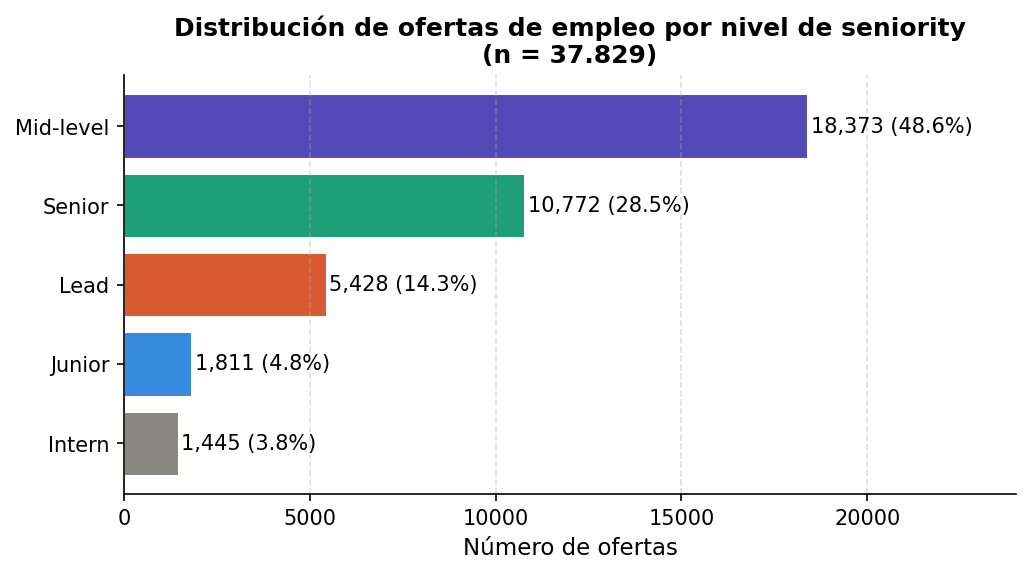
\includegraphics[width=0.75\textwidth]{figures/fig33_dist_seniority}
  \caption{Distribución de las 37.829 ofertas por nivel de \textit{seniority}, inferido mediante reglas léxicas sobre título y descripción de la oferta.}
  \label{fig:dist_seniority}
\end{figure}

\begin{figure}[H]
  \centering
  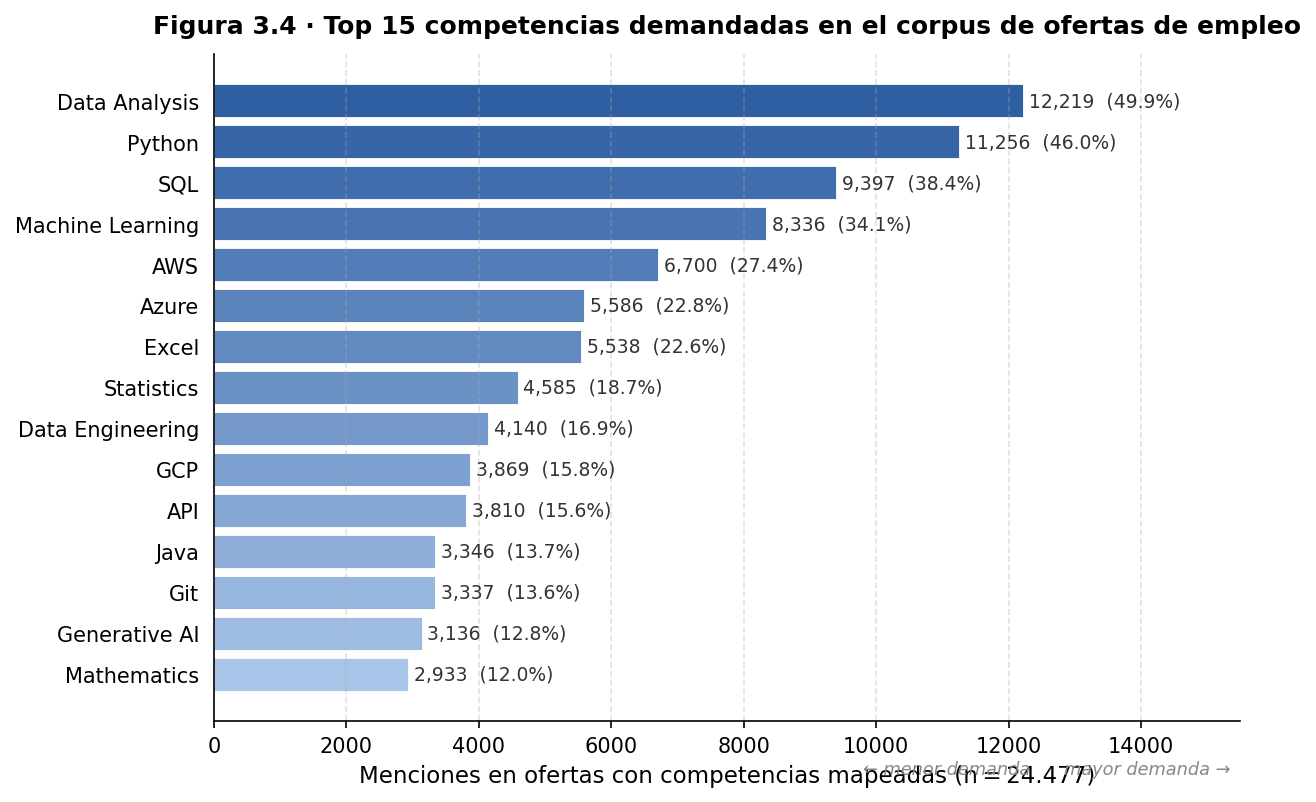
\includegraphics[width=0.88\textwidth]{figures/fig34_top_skills}
  \caption{Top 15 competencias más demandadas en el corpus de ofertas, expresadas como porcentaje de las 37.829 ofertas con al menos una competencia mapeada.}
  \label{fig:top_skills}
\end{figure}

\textit{Dataset de cursos online.} El catálogo de cursos integra 89.332 registros procedentes de \texttt{Udemy}, \texttt{Coursera}, \texttt{edX}, \texttt{Udacity}, \texttt{Skillshare} y \texttt{Simplilearn}. La Tabla~\ref{tab:vars_cursos} describe las variables disponibles.

\begin{table}[H]
  \caption{Diccionario de variables del \textit{dataset} de cursos \textit{online} (\texttt{courses\_catalog\_clean}, $n$\,=\,89.332).}
  \label{tab:vars_cursos}
  \centering
  \footnotesize
  \begin{tabular}{|p{3.5cm}|p{2.2cm}|p{1.5cm}|p{7.0cm}|}
    \hline
    \rowcolor{gray!15}
    \textbf{Variable} & \textbf{Tipo} & \textbf{\% Nulos} & \textbf{Descripción y observaciones} \\
    \hline
    \texttt{course\_id}         & Identificador  & 0\,\%   & ID único del curso; clave primaria \\
    \hline
    \texttt{title}              & Texto libre    & 0\,\%   & Título del curso; \textbf{única fuente de extracción de competencias}; densidad informativa variable \\
    \hline
    \texttt{url}                & URL            & 0\,\%   & Enlace directo a la plataforma \\
    \hline
    \texttt{rating}             & Cuantitativa   & 4,1\,\% & Valoración media (0--5); media: 4,39; $\sigma$: 0,32; distribución muy concentrada en valores altos \\
    \hline
    \texttt{num\_reviews}       & Cuantitativa   & 4,1\,\% & Número de reseñas; mediana: 32; media: 473; máx.: 452.973; distribución muy sesgada a la derecha \\
    \hline
    \texttt{duration}           & Texto libre    & 7,1\,\% & Duración declarada en formatos heterogéneos; no normalizable de forma sistemática \\
    \hline
    \texttt{last\_update\_date} & Fecha          & 2,3\,\% & Última actualización del contenido \\
    \hline
  \end{tabular}
\end{table}

Con una media de 4,39 y una desviación típica de 0,32, prácticamente todos los cursos se concentran entre 4,0 y 4,8 puntos, lo que hace que \texttt{rating} sea un discriminador de calidad muy limitado. El campo \texttt{num\_reviews} sigue una distribución log-normal extrema (mediana 32 frente a media 473). El campo \texttt{duration} no es normalizable de forma fiable y no se incorpora al modelo. La limitación más crítica es que el título es la \textbf{única} fuente de extracción de competencias disponible. Esto restringe la cobertura al 15,7\,\% de los cursos, generando 21.329 pares curso--competencia sobre el total del catálogo.

\textit{Dataset de programas de máster.} El catálogo de másteres contiene 3.503 programas de posgrado procedentes de \texttt{Mastersportal.eu} y universidades e instituciones españolas. La Tabla~\ref{tab:vars_masters} describe sus variables.

\begin{table}[H]
  \caption{Diccionario de variables del \textit{dataset} de másteres (\texttt{masters\_catalog\_clean}, $n$\,=\,3.503).}
  \label{tab:vars_masters}
  \centering
  \footnotesize
  \begin{tabular}{|p{3.5cm}|p{2.2cm}|p{1.5cm}|p{7.0cm}|}
    \hline
    \rowcolor{gray!15}
    \textbf{Variable} & \textbf{Tipo} & \textbf{\% Nulos} & \textbf{Descripción y observaciones} \\
    \hline
    \texttt{master\_id}     & Identificador  & 0\,\%   & ID secuencial; clave primaria \\
    \hline
    \texttt{program\_name}  & Texto libre    & 0\,\%   & Nombre del programa; alta variabilidad de denominación \\
    \hline
    \texttt{university}     & Texto libre    & 0\,\%   & Nombre de la institución; 1.847 valores únicos \\
    \hline
    \texttt{rating}         & Cuantitativa   & 1,4\,\% & Valoración media; escala y fuente variable según agregador \\
    \hline
    \texttt{reviews}        & Cuantitativa   & 1,4\,\% & Número de reseñas; muy disperso entre instituciones \\
    \hline
    \texttt{location}       & Texto libre    & 0\,\%   & Ciudad y país; \textit{online} ($n$\,=\,444), Londres ($n$\,=\,187), Madrid ($n$\,=\,56) \\
    \hline
    \texttt{tuition}        & Texto/Num.     & 3,2\,\% & Matrícula en texto libre; convertido a euros/año en el ETL \\
    \hline
    \texttt{duration}       & Texto libre    & 2,1\,\% & Duración declarada; media estimada: 16 meses \\
    \hline
    \texttt{url}            & URL            & 0\,\%   & Enlace al programa en \texttt{Mastersportal} \\
    \hline
    \texttt{study\_content} & Texto libre    & 0\,\%   & Descripción del plan de estudios; \textbf{fuente principal de extracción de competencias}; longitud media: 312 palabras \\
    \hline
  \end{tabular}
\end{table}

A diferencia de los cursos, los másteres disponen del campo \texttt{study\_content}, con detalle terminológico suficiente para la extracción de competencias. Esto explica la diferencia de cobertura: el 67,6\,\% de los másteres (2.369 programas) presenta al menos una competencia mapeada, con una media de 2,4 competencias por programa, frente al 15,7\,\% de los cursos.

La taxonomía de competencias que articula este enriquecimiento se amplió de 59 a 71 competencias y de 190 a 477 \textit{aliases} (Sección~\ref{subsubsec:extraccion_competencias}), lo que permitió incorporar herramientas relevantes (\texttt{Kafka}, \texttt{Terraform}, \texttt{MLflow}, \texttt{Linux}/\texttt{bash}, \texttt{FastAPI}) y mejorar la cobertura de \textit{aliases} en español.

\textbf{Valoración frente al objetivo.} El objetivo 1 queda cubierto: se dispone de tres \textit{datasets} representativos, limpios, normalizados y enriquecidos semánticamente mediante una taxonomía común, con un \textit{pipeline} ETL documentado y reproducible (Sección~\ref{subsec:proceso_etl}). La limitación identificada --la baja cobertura de competencias en el catálogo de cursos (15,7\,\%), derivada de que el título es la única fuente textual disponible-- se retoma en la Discusión.

% -----------------------------------------------------------
\subsection{Resultados frente al objetivo 2: actualización y definición continua}
\label{subsec:resultados_obj2}
% -----------------------------------------------------------
El segundo objetivo específico exigía establecer un proceso de actualización continua mediante \textit{scraping} periódico de ofertas, másteres y cursos, de forma que los requisitos de competencias y las recomendaciones reflejen el estado real del mercado en cada momento.

El \textit{pipeline} de \textit{scraping} incremental descrito en la Sección~\ref{subsec:pipeline_scraping} estuvo operativo durante los 71 días del período de construcción del sistema (11 de marzo -- 22 de mayo de 2026), ejecutando 187 ciclos repartidos en 9 jornadas activas de recolección (promedio de 20,8 ciclos por jornada). La Tabla~\ref{tab:resumen_scraping} resume los resultados operativos del proceso.

\begin{table}[H]
  \caption{Resultados operativos del \textit{pipeline} de \textit{scraping} incremental frente al objetivo 2.}
  \label{tab:resumen_scraping}
  \centering
  \footnotesize
  \begin{tabular}{|p{7.5cm}|p{5.5cm}|}
    \hline
    \rowcolor{gray!15}
    \textbf{Indicador} & \textbf{Valor} \\
    \hline
    Período de ejecución & 11 mar. -- 22 may. 2026 (71 días) \\
    \hline
    Ciclos de \textit{scraping} ejecutados & 187 (9 jornadas activas; media 20,8/jornada) \\
    \hline
    Registros recuperados por ciclo & Media 312; mediana 270; rango 10--2.100 \\
    \hline
    Registros brutos acumulados & 58.408 \\
    \hline
    Recapturas inter-ciclo descartadas & 17.629 (30,2\,\%) \\
    \hline
    Umbral de antigüedad admitido & 30 días (justificado por Burning Glass Technologies et al., 2017) \\
    \hline
    Cobertura temporal del \textit{snapshot} final & feb. 2024 -- may. 2026 (mayor densidad oct. 2025 -- may. 2026) \\
    \hline
  \end{tabular}
\end{table}

La deduplicación basada en URL (y, en su defecto, en la combinación portal--título--empresa--localización) descartó el 30,2\,\% de los registros brutos como recapturas entre ciclos, lo que confirma que el mecanismo incremental evita la acumulación de duplicados pese a la naturaleza solapada de las consultas sucesivas. La Figura~\ref{fig:evolucion_temporal} muestra la evolución mensual del volumen de ofertas recopiladas: tras una fase de recolección intensiva con un máximo de 18.665 ofertas en febrero de 2026, el volumen se estabiliza entre 1.750 y 2.155 ofertas mensuales durante el período de mantenimiento incremental (abril--mayo de 2026), lo que es coherente con un régimen de actualización periódica en estado estacionario.

Sobre los 40.779 registros únicos resultantes tras descartar las recapturas, el proceso ETL descrito en la Sección~\ref{subsec:proceso_etl} aplicó una segunda fase de limpieza y enriquecimiento. La Tabla~\ref{tab:etl_impacto} resume el impacto cuantitativo conjunto del \textit{pipeline} de \textit{scraping} y del proceso ETL sobre el \textit{dataset} de ofertas de empleo.

\begin{table}[H]
  \caption{Impacto cuantitativo del \textit{pipeline} de \textit{scraping} y del proceso ETL sobre el \textit{dataset} de ofertas de empleo.}
  \label{tab:etl_impacto}
  \centering
  \footnotesize
  \begin{tabular}{|p{7.5cm}|p{5.5cm}|}
    \hline
    \rowcolor{gray!15}
    \textbf{Indicador} & \textbf{Valor} \\
    \hline
    Registros brutos totales (suma de 187 ciclos) & 58.408 \\
    \hline
    Recapturas inter-ciclo eliminadas durante fusión incremental & 17.629 (30,2\,\%) \\
    \hline
    Registros únicos en acumulador pre-ETL & 40.779 \\
    \hline
    Duplicados por URL eliminados en ETL & 2.723 (6,7\,\%) \\
    \hline
    Registros descartados por descripción ausente & 6.812 (16,7\,\%) \\
    \hline
    Registros eliminados total por ETL (desde acumulador) & 2.950 (7,2\,\%) \\
    \hline
    Registros finales limpios & \textbf{37.829} \\
    \hline
    Fuentes integradas (portales de empleo) & 3 (\texttt{Indeed}, \texttt{LinkedIn}, \texttt{Glassdoor}) \\
    \hline
    \% nulos en \texttt{job\_level} / \texttt{job\_function} & 84,5\,\% (variables derivadas por reglas léxicas) \\
    \hline
    \% nulos en \texttt{company} & 1,8\,\% \\
    \hline
    \% nulos en \texttt{date\_posted} & 1,3\,\% \\
    \hline
    \% nulos en \texttt{location} & 3,6\,\% \\
    \hline
    Valores imputados & 0\,\% (no se aplica imputación) \\
    \hline
    \textit{Skills} extraídas (pares oferta--competencia) & 134.056 \\
    \hline
    \% valores normalizados & Duraciones a meses (cobertura parcial); precios de másteres a euros/año (96,8\,\% con precio disponible) \\
    \hline
    Variables derivadas añadidas & \texttt{role\_family}, \texttt{seniority}, \texttt{work\_mode}, \texttt{employment\_type} \\
    \hline
  \end{tabular}
\end{table}

Los valores ausentes que persisten tras el ETL se conservan sin imputación: los portales no exponen estos campos en sus páginas públicas de forma sistemática, de modo que su ausencia es una limitación inherente a la fuente original, no corregible mediante técnicas de imputación sin introducir sesgos.

\textbf{Valoración frente al objetivo.} El objetivo 2 queda cubierto: el \textit{pipeline} incremental ha operado de forma sostenida durante 71 días, ha incorporado únicamente novedades reales (descartando recapturas) y ha mantenido el \textit{snapshot} actualizado hasta mayo de 2026. La transición observada entre la fase de recolección intensiva y la fase de mantenimiento (Figura~\ref{fig:evolucion_temporal}) constituye evidencia directa de que el sistema sostiene una cadencia de actualización periódica, tal como requiere el objetivo. Queda abierta, y se discute más adelante, la cuestión de la cadencia óptima a largo plazo y de la fiabilidad de las fuentes ante cambios en su estructura.

% -----------------------------------------------------------
\subsection{Resultados frente al objetivo 3: motor de recomendación y mecanismo de ajuste a rol}
\label{subsec:resultados_obj3}
% -----------------------------------------------------------
El tercer objetivo específico exigía diseñar e implementar un motor de recomendación para formación y empleo, comparando distintas aproximaciones de \textit{scoring} e incorporando un mecanismo que evite recomendar roles para los que el perfil del candidato no esté aún preparado.

\textbf{Comparación de variantes de \textit{scoring}.} Aplicando el protocolo de evaluación automática descrito en la Sección~\ref{subsec:evaluacion_modelo} (esquema de \textit{holdout} interno 80/20, combinando cobertura léxica y similitud semántica), la Tabla~\ref{tab:tabla3_9} resume la comparación entre las cuatro variantes evaluadas sobre $n$\,=\,482 candidatos (de los 500 CVs del corpus de validación, 18 fueron excluidos por presentar menos de cuatro competencias extraídas).

\begin{table}[H]
  \caption{Resultados del estudio de ablación por variante. Objetivo: $0{,}6 \times \textit{Recall} + 0{,}4 \times \textit{Gap\_reduction}$.}
  \label{tab:tabla3_9}
  \centering
  \footnotesize
  \begin{tabular}{|p{3.6cm}|c|c|c|c|c|}
    \hline
    \rowcolor{gray!15}
    \textbf{Variante} & \boldmath{$\alpha_{\text{cov}}$} & \boldmath{$\alpha_{\text{sem}}$} & \textbf{\textit{Recall}} & \textbf{\textit{Gap red.}} & \textbf{Objetivo} \\
    \hline
    \textbf{\texttt{balanced\_50\_50}} & \textbf{0{,}50} & \textbf{0{,}50} & \textbf{0{,}413} & \textbf{0{,}750} & \textbf{0{,}548} \\
    \hline
    \texttt{hybrid\_tuned}    & 0{,}65 & 0{,}35 & 0{,}412 & 0{,}749 & 0{,}547 \\
    \hline
    \texttt{semantic\_only}   & 0{,}00 & 1{,}00 & 0{,}410 & 0{,}732 & 0{,}539 \\
    \hline
    \texttt{coverage\_only}   & 1{,}00 & 0{,}00 & 0{,}406 & 0{,}738 & 0{,}539 \\
    \hline
  \end{tabular}
  \\\smallskip
  {\footnotesize $n$\,=\,482 candidatos (de 500 CVs totales; 18 excluidos por tener menos de 4 competencias extraídas); protocolo \textit{holdout} 80/20; semilla aleatoria fijada por candidato.}
\end{table}

\begin{figure}[H]
  \centering
  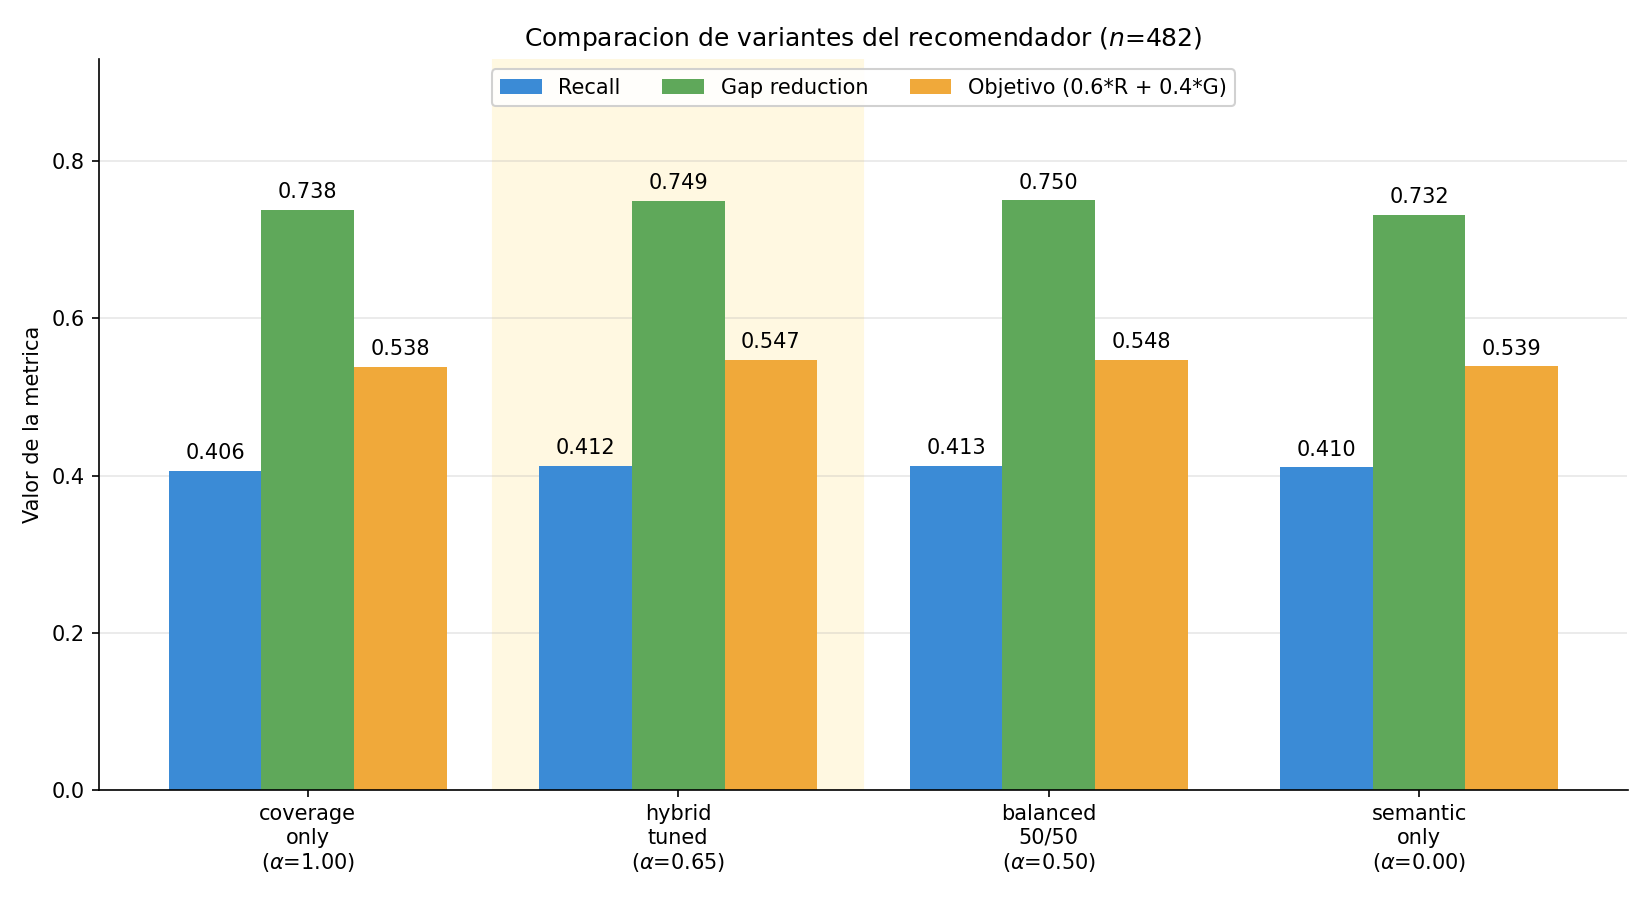
\includegraphics[width=0.85\textwidth]{figures/fig36_ablacion}
  \caption{Comparación de variantes del recomendador en el estudio de ablación ($n$\,=\,482). Función objetivo: $0{,}6 \times \textit{recall} + 0{,}4 \times \textit{gap\_reduction}$.}
  \label{fig:ablacion}
\end{figure}

\begin{figure}[H]
  \centering
  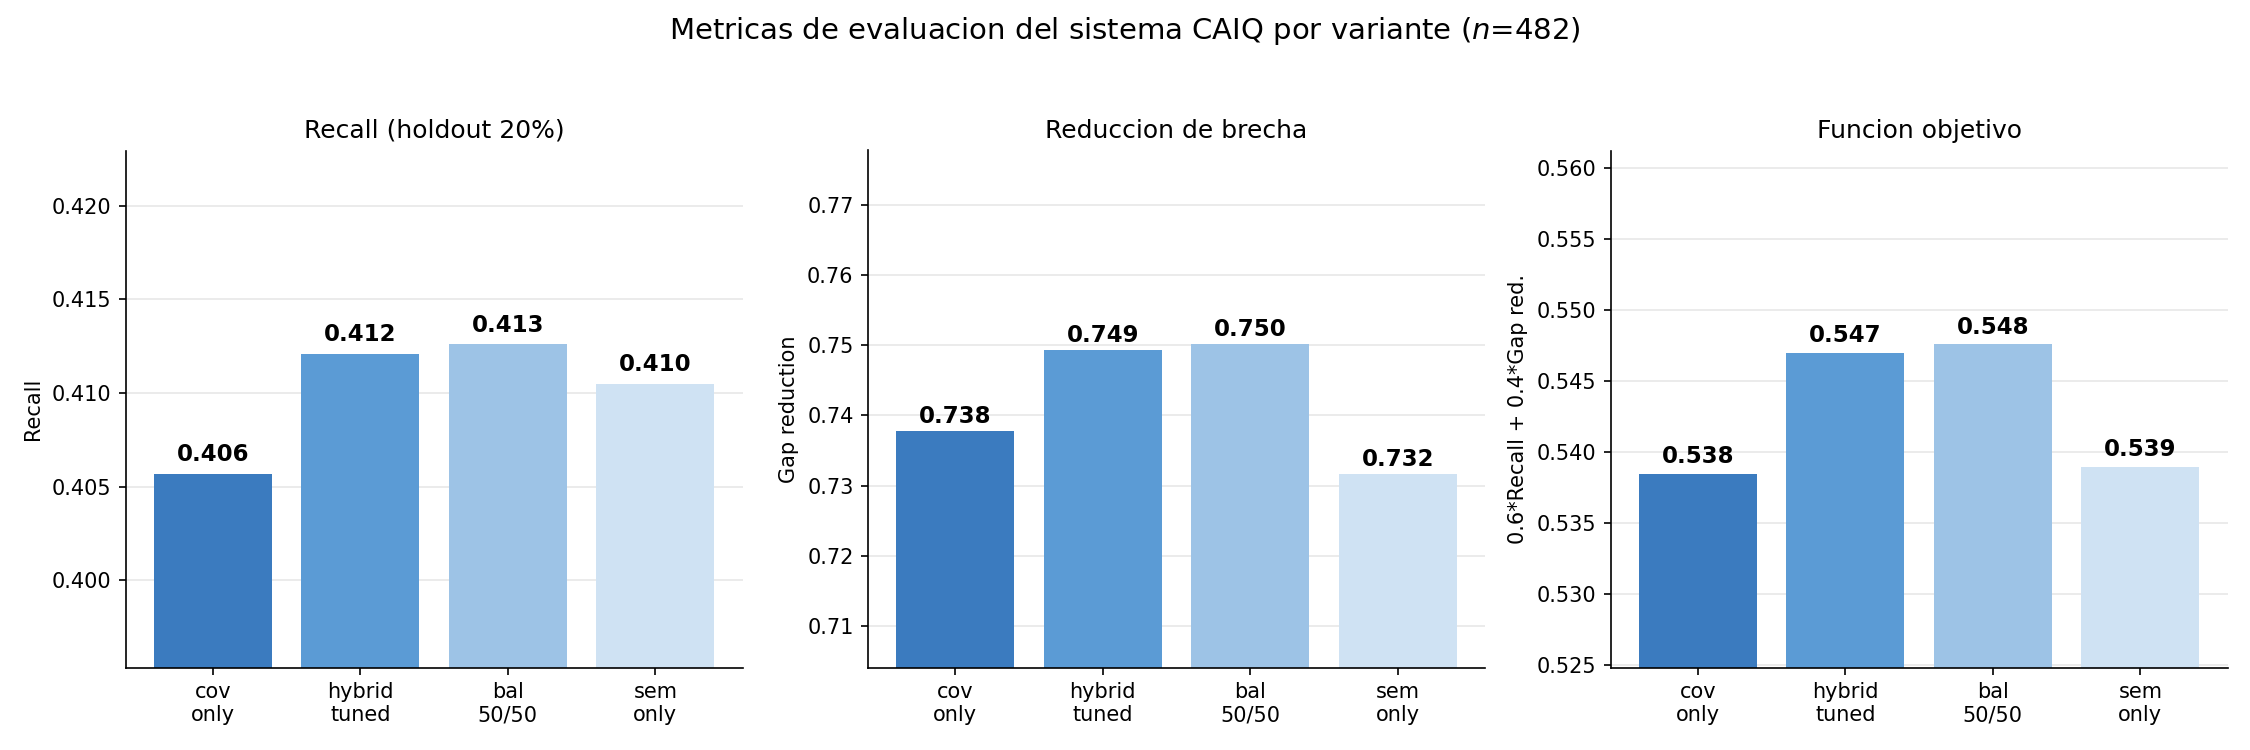
\includegraphics[width=0.85\textwidth]{figures/fig37_metricas_modelo}
  \caption{Métricas de evaluación del sistema CAIQ por variante: \textit{recall}, reducción de brecha y función objetivo compuesta ($n$\,=\,482).}
  \label{fig:metricas}
\end{figure}

Las cuatro variantes evaluadas (\texttt{balanced\_50\_50}, \texttt{hybrid\_tuned}, \texttt{semantic\_only} y \texttt{coverage\_only}) obtienen un \textit{recall} entre 0,406 y 0,413 y una reducción del \textit{gap} entre 0,732 y 0,750, con una diferencia máxima de solo 0,009 en la función objetivo compuesta ($0{,}6 \times \textit{recall} + 0{,}4 \times \textit{gap\_reduction}$), como muestran las Figuras~\ref{fig:ablacion} y~\ref{fig:metricas}. Esto indica que ni la cobertura léxica ni la similitud semántica por separado dominan claramente sobre el conjunto ampliado de candidatos. La variante desplegada en producción, \texttt{hybrid\_tuned} ($\alpha_{\text{cov}}=0{,}65$, $\alpha_{\text{sem}}=0{,}35$), obtiene un \textit{recall} de 0,412 y una reducción de \textit{gap} de 0,749 (objetivo\,=\,0,547), prácticamente empatada con la mejor variante (\texttt{balanced\_50\_50}, objetivo\,=\,0,548) y por delante de las dos variantes puras. Este resultado contrasta con el obtenido sobre la muestra reducida inicial ($n$\,=\,15), donde \texttt{coverage\_only} aparecía como claramente superior; al ampliar el corpus de evaluación a 482 candidatos reales, esa ventaja se diluye y las diferencias entre variantes dejan de ser determinantes. Dado que la diferencia entre las cuatro configuraciones es marginal, se mantiene \texttt{hybrid\_tuned} como variante de producción por conservar tanto la señal de cobertura léxica directa como la componente semántica, que permite capturar afinidades entre competencias relacionadas que el \textit{matching} léxico estricto no detectaría (Burke, 2002).

Desde un punto de vista práctico, esta convergencia de resultados constituye en sí misma un hallazgo relevante: indica que el rendimiento global del recomendador es robusto frente a la elección de ponderación entre cobertura léxica y similitud semántica, por lo que dicha elección no constituye un factor crítico de riesgo para el sistema. Esto simplifica el mantenimiento del modelo, ya que ajustes futuros de $\alpha_{\text{cov}}$ y $\alpha_{\text{sem}}$ pueden realizarse con un impacto acotado y predecible sobre la calidad de las recomendaciones.

\textbf{Mecanismo de ajuste y anti-recomendación de roles no preparados.} El segundo componente del objetivo --evitar recomendar roles para los que el candidato no está preparado-- se resuelve mediante el cálculo del \texttt{role\_fit\_score} y la cobertura ponderada por bandas (\texttt{coverage\_core}, \texttt{coverage\_important}, \texttt{coverage\_complementary}), descritos en la Sección~\ref{subsubsec:calculo_gap_detalle}. Para cada familia de rol, el sistema calcula el \textit{gap} de competencias respecto al perfil objetivo (Tabla~\ref{tab:tabla3_7}) y pondera de forma diferenciada las carencias \textit{core}, \textit{important} y \textit{complementary}. Un perfil con \textit{gap} concentrado en la banda \textit{core} de un rol --es decir, con baja \texttt{coverage\_core}-- obtiene un \texttt{role\_fit\_score} bajo para ese rol, lo que el sistema traduce operativamente en: (a) no presentar ese rol como \texttt{detected\_best\_role} ni como destino prioritario de recomendaciones de empleo, y (b) priorizar en su lugar recursos formativos (másteres y cursos) que cubran específicamente las competencias \textit{core} del \textit{gap}, antes de sugerir ofertas de empleo para ese rol. De este modo, el mecanismo de \textit{scoring} y el de ajuste por bandas operan de forma conjunta: el primero ordena los recursos formativos y de empleo por relevancia, y el segundo determina si, dado el estado actual del perfil, resulta pertinente recomendar directamente un rol o, en su lugar, recomendar primero la formación necesaria para alcanzarlo.

\textbf{Valoración frente al objetivo.} El objetivo 3 queda cubierto: se han implementado y comparado cuatro variantes de \textit{scoring} sobre una muestra robusta de 482 candidatos reales, seleccionando \texttt{hybrid\_tuned} como variante de producción por mantener tanto la señal de cobertura léxica como la semántica; y se ha implementado el mecanismo de \texttt{role\_fit\_score} y cobertura por bandas que opera como filtro de pertinencia, evitando recomendar roles para los que el candidato presenta carencias estructurales (\textit{core}) sin cubrir. La convergencia de resultados entre variantes (diferencia máxima de 0,009) indica que la elección de ponderación no es un factor crítico de riesgo, lo que se discute con más detalle en el capítulo siguiente junto con el margen de mejora que representa un \textit{recall} absoluto de 0,412.

% -----------------------------------------------------------
\subsection{Resultados frente al objetivo 4: validación cuantitativa y sobre casos de uso}
\label{subsec:resultados_obj4}
% -----------------------------------------------------------
El cuarto objetivo específico exigía evaluar la cobertura y coherencia del sistema mediante métricas cuantitativas y validación sobre casos de uso representativos.

\textbf{Validación cuantitativa del módulo de extracción.} La validación se realizó sobre los 500 CVs del corpus de validación (499 evaluados; 1 excluido por texto vacío), combinando 14 CVs reales anonimizados y 486 CVs sintéticos. Para 88 CVs del corpus original se dispone de anotaciones manuales de \textit{skills} esperadas, construidas mediante revisión humana de cada documento; para los 412 CVs adicionales no existe anotación manual, por lo que se generaron anotaciones automáticas extrayendo las competencias mencionadas en la sección de habilidades técnicas de cada documento y contrastándolas con la taxonomía controlada del sistema. El sistema se evaluó frente a ambas anotaciones; los resultados se presentan desglosados por tipo de anotación, ya que --como se discute más abajo-- ambas miden aspectos distintos del comportamiento del parser y no son directamente comparables entre sí.

La Tabla~\ref{tab:tabla3_6} muestra que, sobre el subconjunto de referencia con anotación manual ($n$\,=\,87), el sistema obtiene una precisión micro de 0,698, un \textit{recall} micro de 0,995 y un F1 de 0,820 (1.114 verdaderos positivos, 482 falsos positivos, 6 falsos negativos). La Figura~\ref{fig:cv_parser} muestra la distribución por CV de estas tres métricas.

\begin{figure}[H]
  \centering
  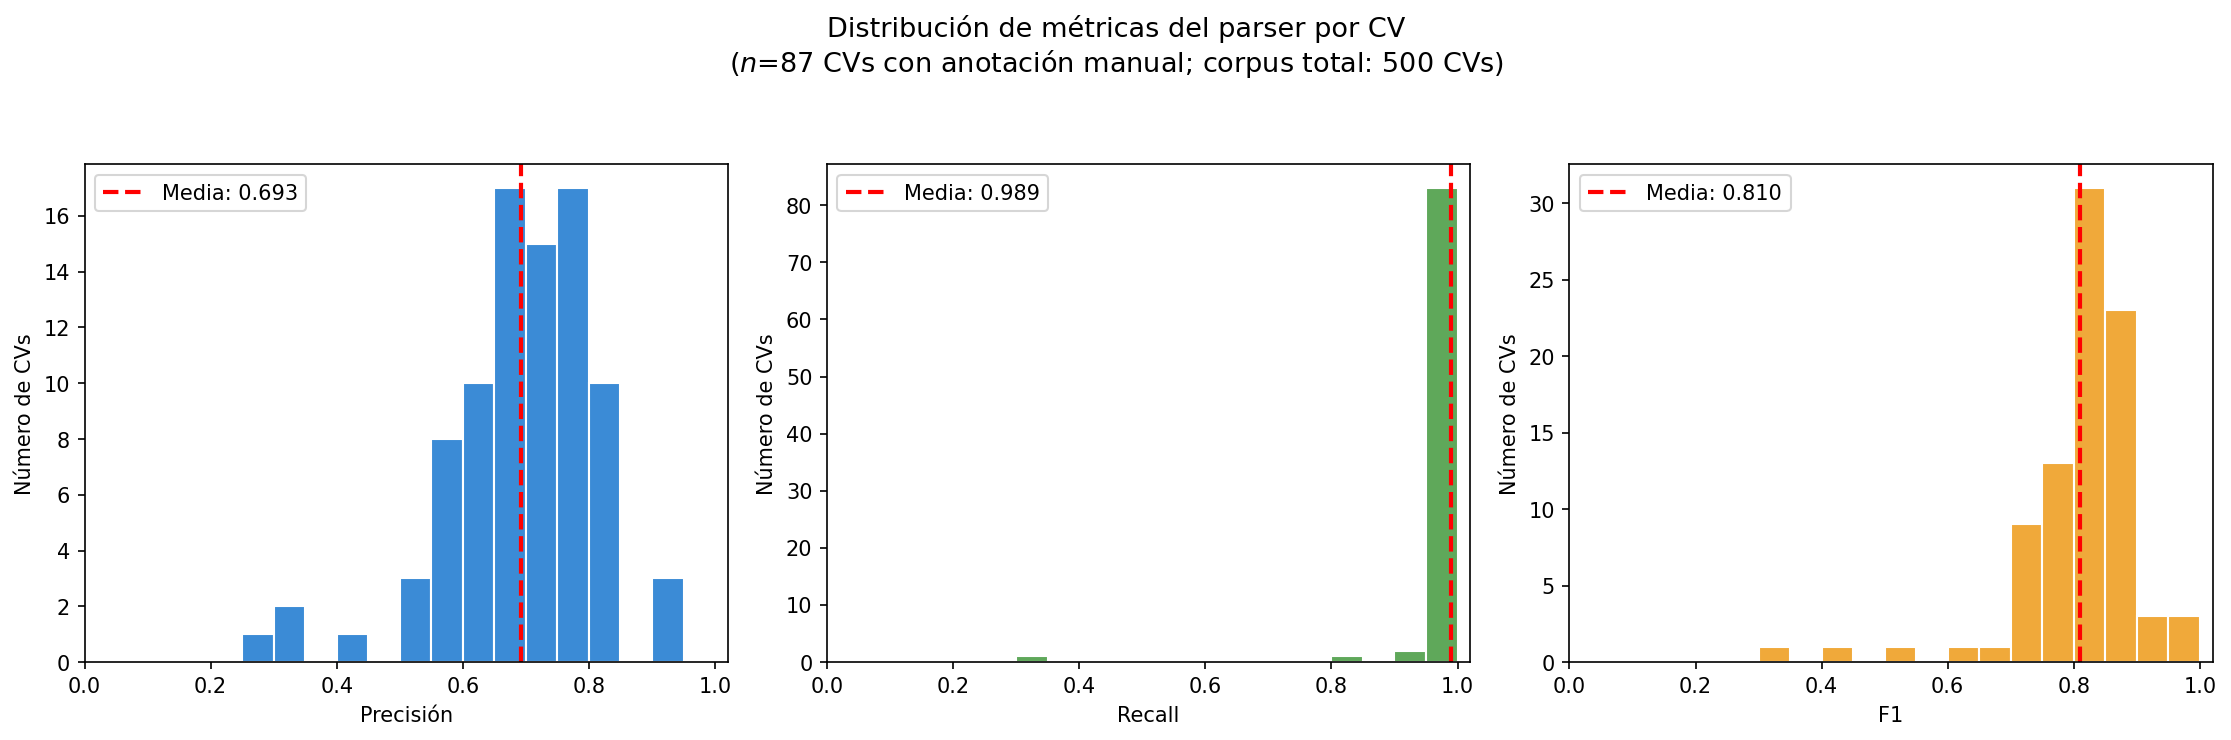
\includegraphics[width=0.85\textwidth]{figures/fig38_cv_parser_metrics}
  \caption{Distribución de precisión, \textit{recall} y F1 por CV en la validación manual del módulo de extracción ($n$\,=\,87 CVs con anotación manual; corpus total: 500 CVs).}
  \label{fig:cv_parser}
\end{figure}

\begin{table}[H]
  \caption{Resultados de la validación manual del módulo de extracción sobre CVs anonimizados.}
  \label{tab:tabla3_6}
  \centering
  \footnotesize
  \begin{tabular}{|l|c|c|c|c|}
    \hline
    \rowcolor{gray!15}
    \textbf{Agregación} & \textbf{Precisión} & \textbf{\textit{Recall}} & \textbf{F1} & \textbf{TP / FP / FN} \\
    \hline
    Micro & 0{,}698 & 0{,}995 & 0{,}820 & 1114 / 482 / 6 \\
    Macro & 0{,}693 & 0{,}989 & 0{,}810 & --- \\
    \hline
  \end{tabular}
  \\\smallskip
  {\footnotesize $n$\,=\,87 CVs con anotación manual (de un corpus total de 500 CVs). Media de \textit{skills} esperadas por CV: 12,87; media detectadas: 18,34.}
\end{table}

El \textit{recall} micro de 0,995 indica que el sistema recupera prácticamente todas las competencias esperadas. La precisión de 0,698 refleja la presencia de falsos positivos, consecuencia de la lógica de detección amplia de la taxonomía; este valor es ligeramente inferior al obtenido en la validación inicial (0,728), atribuible a la ampliación de la taxonomía de 59 a 71 competencias y a los nuevos \textit{aliases} en español incorporados para mejorar la cobertura sobre CVs redactados en castellano.

\textbf{Validación extendida sobre el corpus completo de 500 CVs.} Para comprobar que este resultado generaliza más allá de los 87 CVs de referencia, se extendió la validación a los 412 CVs restantes del corpus mediante la anotación automática descrita anteriormente. La Tabla~\ref{tab:tabla3_6b} y la Figura~\ref{fig:validacion_500} resumen los resultados por subconjunto.

\begin{table}[H]
  \caption{Validación extendida del módulo de extracción sobre el corpus completo de 500 CVs, desglosada por tipo de anotación.}
  \label{tab:tabla3_6b}
  \centering
  \footnotesize
  \begin{tabular}{|l|c|c|c|c|c|c|}
    \hline
    \rowcolor{gray!15}
    \textbf{Subconjunto} & \textbf{$n$} & \textbf{Precisión} & \textbf{\textit{Recall}} & \textbf{F1} & \textbf{Media esp.} & \textbf{Media det.} \\
    \hline
    Manual (referencia)       & 87  & 0{,}698 & 0{,}995 & 0{,}820 & 12{,}87 & 18{,}34 \\
    \hline
    Auto (sección Habilidades) & 392 & 0{,}552 & 0{,}969 & 0{,}703 & 8{,}66  & 15{,}19 \\
    \hline
    Sin habilidades auto-extraídas & 20 & --- & --- & --- & 0{,}00 & 3{,}75 \\
    \hline
    Excluido (texto vacío)    & 1   & --- & --- & --- & --- & --- \\
    \hline
  \end{tabular}
  \\\smallskip
  {\footnotesize Precisión, \textit{recall} y F1 son valores micro. Para el subconjunto ``Sin habilidades auto-extraídas'' no existen competencias esperadas (sección de habilidades sin coincidencias con la taxonomía), por lo que precisión y \textit{recall} no son computables; estos 20 CVs corresponden a perfiles ajenos al ámbito de datos y se analizan a continuación desde la perspectiva de los falsos positivos.}
\end{table}

\begin{figure}[H]
  \centering
  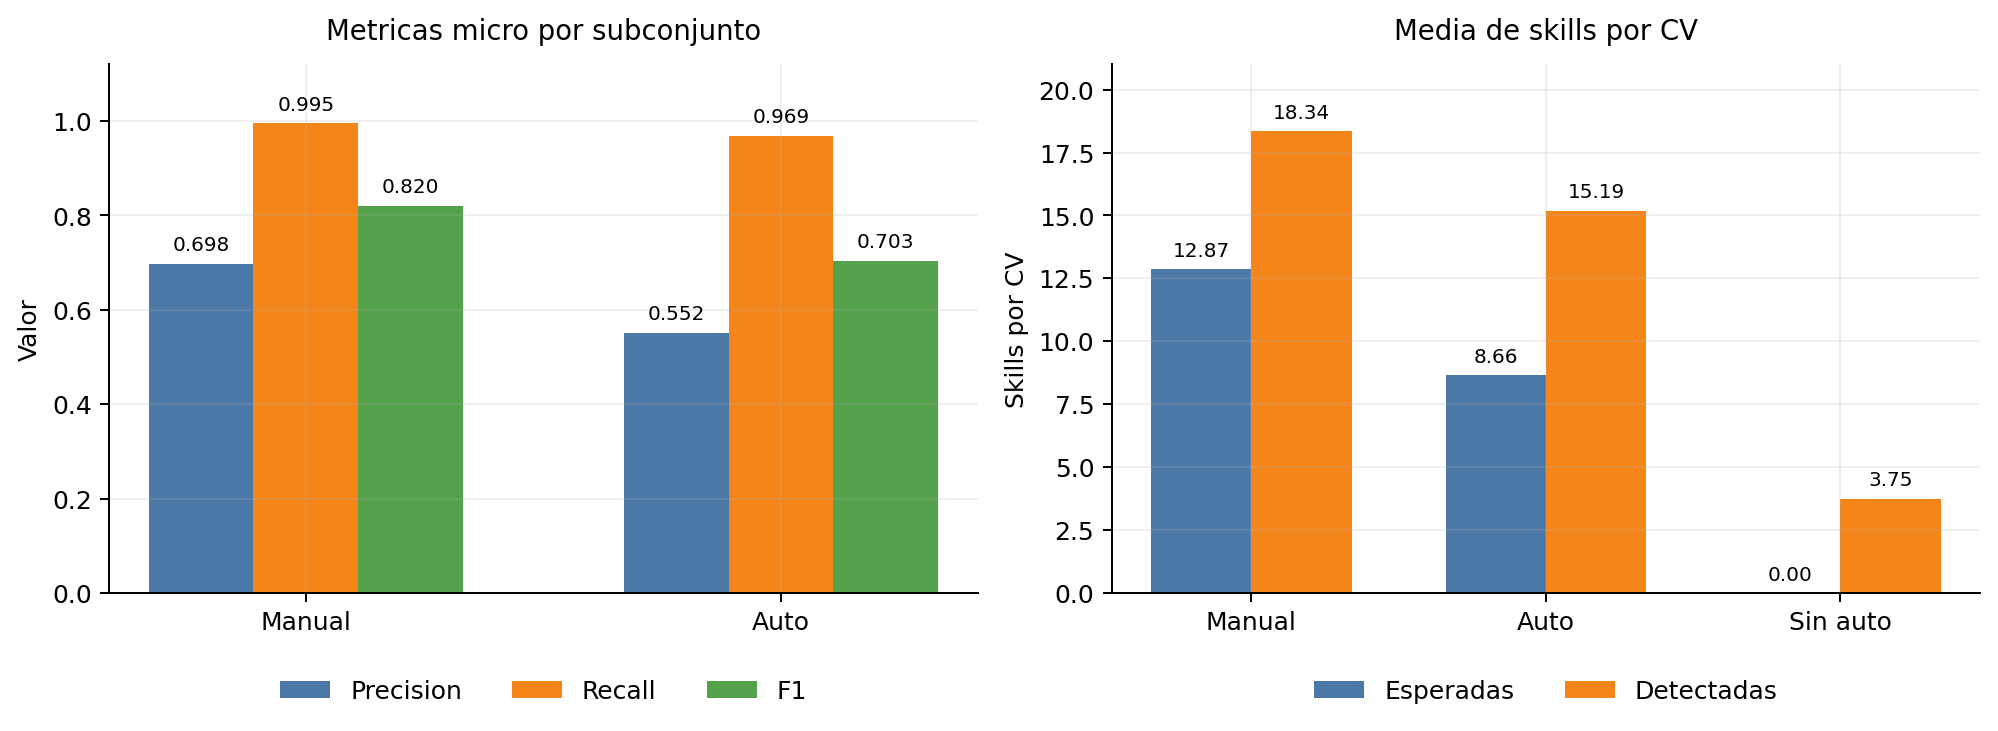
\includegraphics[width=0.95\textwidth]{figures/fig39_validacion_500cvs}
  \caption{Validación extendida del parser sobre el corpus de 500 CVs: métricas micro por tipo de anotación (izquierda) y media de \textit{skills} esperadas frente a detectadas por subconjunto (derecha).}
  \label{fig:validacion_500}
\end{figure}

El \textit{recall} se mantiene alto y estable entre el subconjunto manual (0,995) y el subconjunto auto-anotado (0,969), lo que confirma que la capacidad del parser para recuperar las competencias relevantes generaliza al corpus ampliado y no es un artefacto de los 87 CVs de referencia. Tras corregir la extracción de la sección de habilidades, el número de CVs auto-anotados evaluables aumenta de 166 a 392 y la precisión micro del subconjunto auto-anotado sube de 0,227 a 0,552. Esta mejora indica que la baja precisión anterior estaba parcialmente inducida por una referencia automática incompleta; aun así, la precisión auto-anotada sigue sin ser directamente comparable con la del subconjunto manual, porque la referencia automática solo recoge competencias mencionadas explícitamente en la sección de habilidades del CV (media de 8,66 \textit{skills} esperadas por documento), mientras que el parser detecta también competencias presentes en la experiencia, los proyectos y la formación (media de 15,19 detectadas), tal y como está diseñado para hacer (Sección~\ref{subsubsec:extraccion_competencias}). Por este motivo, las cifras de precisión reportadas como referencia principal del sistema (Tabla~\ref{tab:tabla3_6}) son las del subconjunto con anotación manual ($n$\,=\,87), construido por revisión humana completa de cada CV y, por tanto, sensible a competencias mencionadas en cualquier sección del documento.

\textbf{Validación sobre casos de uso representativos.} El corpus de 500 CVs combina 14 CVs reales anonimizados y 486 CVs sintéticos que cubren perfiles de distintos roles de datos (\textit{data analyst}, \textit{data scientist}, \textit{data engineer}, \textit{ml\_engineer}), niveles de \textit{seniority} (\textit{intern} a \textit{lead}) e idiomas (español e inglés). Adicionalmente, 20 CVs corresponden a perfiles ajenos al ámbito de datos (por ejemplo, sanidad, derecho, recursos humanos), sin competencias esperadas de la taxonomía; estos casos se utilizan para evaluar el comportamiento del sistema ante perfiles fuera de dominio, con una media de 3,75 competencias detectadas por CV frente a 0 esperadas. En conjunto, estos 500 casos constituyen el banco de pruebas representativo exigido por el objetivo, cubriendo tanto los perfiles para los que el sistema fue diseñado como los casos límite de perfiles no orientados a datos.

La Tabla~\ref{tab:resumen_validacion} sintetiza los resultados de validación frente al objetivo 4.

\begin{table}[H]
  \caption{Síntesis de los resultados de validación frente al objetivo 4.}
  \label{tab:resumen_validacion}
  \centering
  \footnotesize
  \begin{tabular}{|p{4.5cm}|p{1.2cm}|p{2.0cm}|p{2.0cm}|p{2.0cm}|p{2.0cm}|}
    \hline
    \rowcolor{gray!15}
    \textbf{Subconjunto} & \textbf{$n$} & \textbf{Precisión} & \textbf{\textit{Recall}} & \textbf{F1} & \textbf{Media det.} \\
    \hline
    Manual (referencia)               & 87  & 0{,}698 & 0{,}995 & 0{,}820 & 18{,}34 \\
    \hline
    Auto (sección Habilidades)        & 392 & 0{,}552 & 0{,}969 & 0{,}703 & 15{,}19 \\
    \hline
    Sin habilidades (fuera de dominio) & 20  & ---     & ---     & ---     & 3{,}75 \\
    \hline
  \end{tabular}
\end{table}

\textbf{Valoración frente al objetivo.} El objetivo 4 queda cubierto: se dispone de métricas cuantitativas de cobertura (\textit{recall}) y precisión sobre un corpus de 500 CVs, con un subconjunto de referencia anotado manualmente, y de una validación sobre casos de uso representativos que incluyen perfiles de distintos roles, niveles de experiencia, idiomas y --como caso límite-- perfiles ajenos al ámbito de datos. La coherencia del sistema queda evidenciada por la estabilidad del \textit{recall} (0,995 y 0,969) entre el subconjunto manual y el ampliado. La precisión moderada (0,698 en el subconjunto de referencia) constituye el principal margen de mejora identificado y se discute en el capítulo siguiente.

% -----------------------------------------------------------
\subsection{Resultados frente al objetivo 5: implementación de la interfaz web}
\label{subsec:resultados_obj5}
% -----------------------------------------------------------
El quinto objetivo específico exigía desplegar una interfaz web funcional orientada a la toma de decisión profesional del candidato.

El sistema se implementó como una aplicación \texttt{Streamlit} desplegada mediante un contenedor Docker en Hugging Face Spaces, de acceso público y sin infraestructura propia (Tabla~\ref{tab:stack}). La aplicación implementa el flujo completo descrito en la arquitectura del sistema (Figura~\ref{fig:arquitectura}): el usuario carga su CV en PDF, DOCX o TXT; el sistema construye su perfil profesional (Sección~\ref{subsec:modelado_cv}); calcula el \textit{skill gap} respecto al rol objetivo (Sección~\ref{subsec:calculo_gap}); y presenta recomendaciones de formación y empleo.

La Figura~\ref{fig:app_resumen} muestra la pantalla de resumen del perfil, donde se presentan las competencias detectadas, el nivel de \textit{seniority} inferido y la puntuación de ajuste a cada familia de rol (\texttt{role\_fit\_scores}). La Figura~\ref{fig:app_skills} muestra el panel de inteligencia de competencias, que desglosa el \textit{skill gap} por bandas (\textit{core}, \textit{important}, \textit{complementary}) para el rol objetivo seleccionado. La Figura~\ref{fig:app_recomendaciones} muestra las tarjetas de recomendación de formación y empleo, con etiquetas de color que identifican qué competencias del \textit{gap} cubre cada recurso (moradas para másteres, azules para cursos), priorizando las competencias \textit{core} sobre las \textit{important} (Sección~\ref{subsubsec:visualizacion_gap}).

\begin{figure}[H]
  \centering
  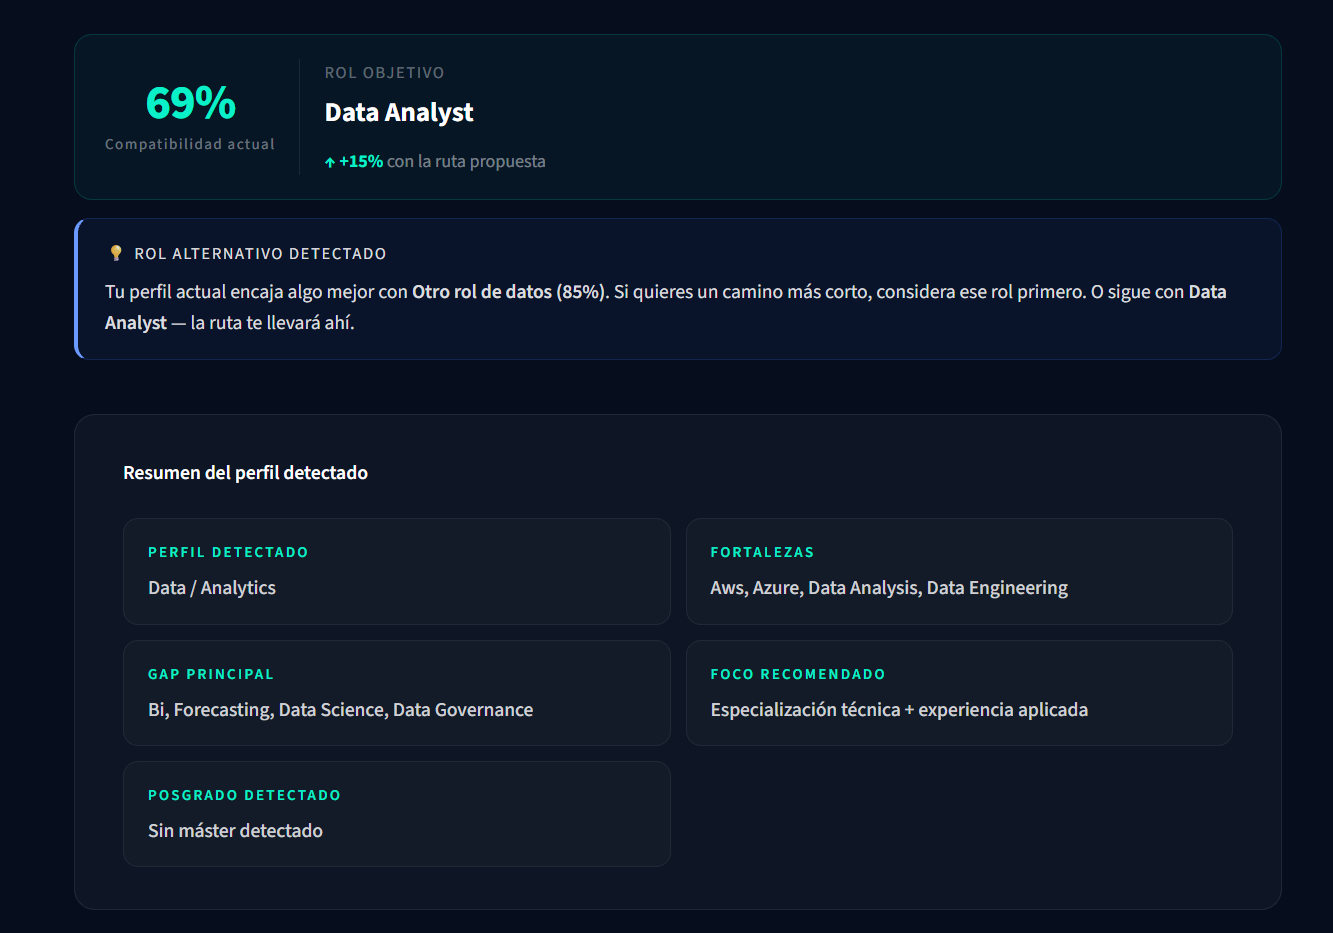
\includegraphics[width=0.85\textwidth]{figures/app_resumen_perfil}
  \caption{Interfaz web del sistema CAIQ: pantalla de resumen del perfil profesional, con competencias detectadas, \textit{seniority} inferido y ajuste por familia de rol.}
  \label{fig:app_resumen}
\end{figure}

\begin{figure}[H]
  \centering
  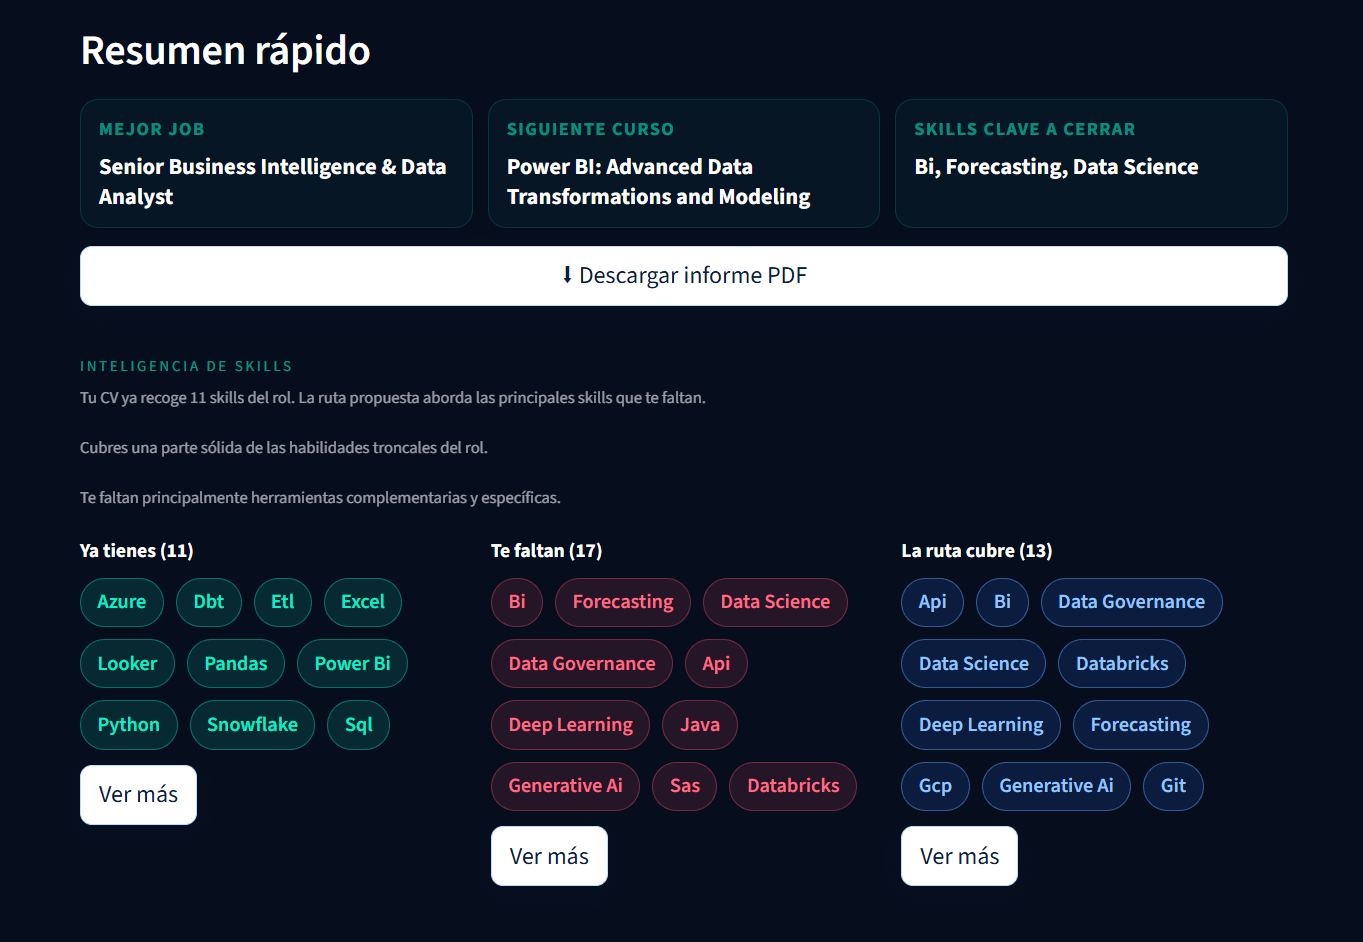
\includegraphics[width=0.85\textwidth]{figures/app_inteligencia_skills}
  \caption{Interfaz web del sistema CAIQ: panel de inteligencia de competencias, con el \textit{skill gap} desglosado por bandas \textit{core}, \textit{important} y \textit{complementary} para el rol objetivo.}
  \label{fig:app_skills}
\end{figure}

\begin{figure}[H]
  \centering
  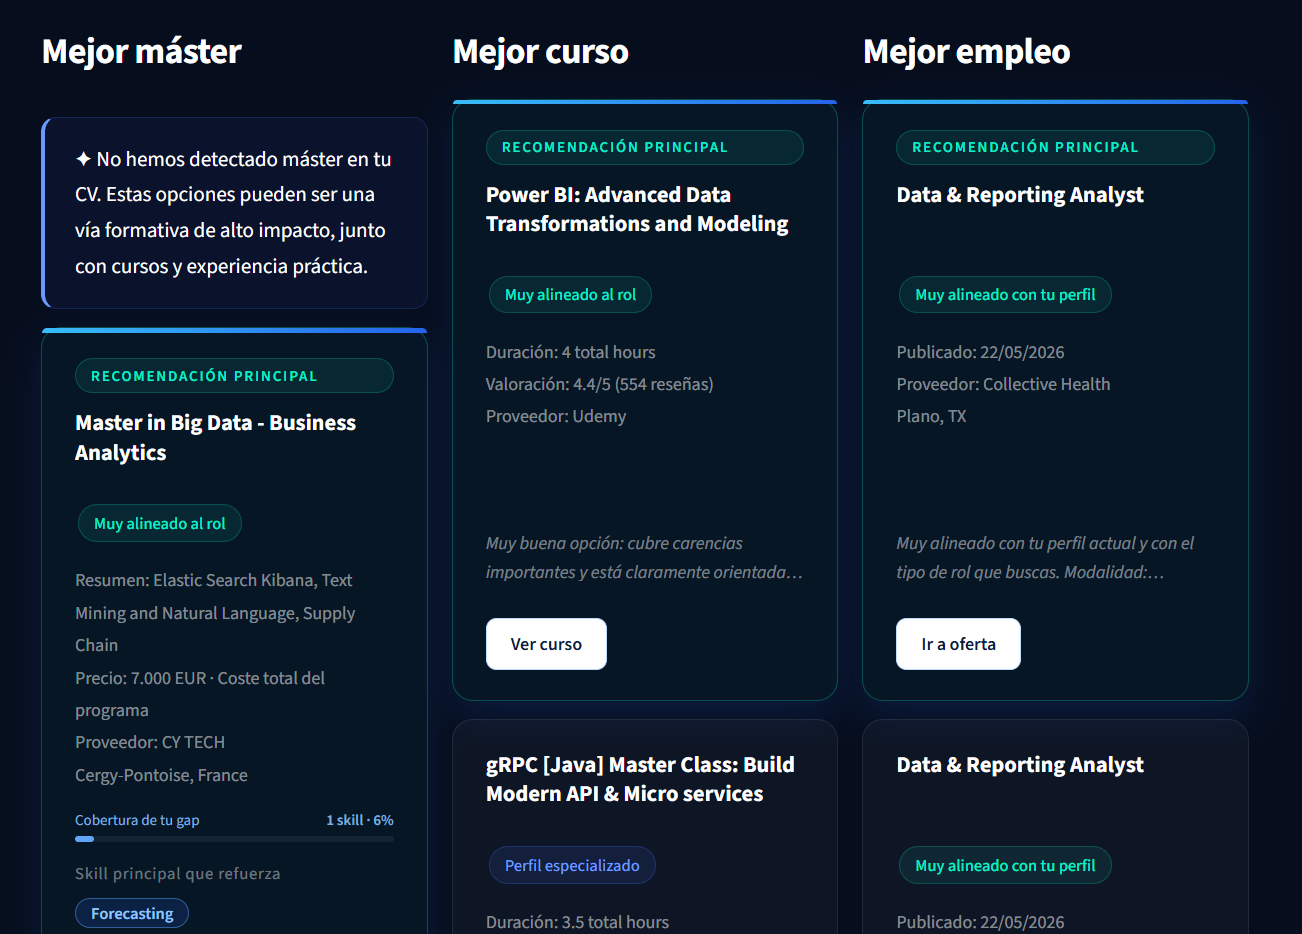
\includegraphics[width=0.85\textwidth]{figures/app_recomendaciones}
  \caption{Interfaz web del sistema CAIQ: tarjetas de recomendación de formación y empleo, con etiquetas que identifican las competencias del \textit{gap} cubiertas por cada recurso.}
  \label{fig:app_recomendaciones}
\end{figure}

\textbf{Valoración frente al objetivo.} El objetivo 5 queda cubierto: la interfaz web está desplegada, es de acceso público y cubre el flujo completo desde la carga del CV hasta la presentación de recomendaciones explicables, integrando de forma visual los resultados de los módulos de extracción, cálculo del \textit{gap} y recomendación descritos en los objetivos anteriores.

% -----------------------------------------------------------
\subsection{Síntesis de resultados}
\label{subsec:sintesis_resultados}
% -----------------------------------------------------------
La Tabla~\ref{tab:sintesis_objetivos} resume el grado de cumplimiento de cada objetivo específico a la luz de los resultados presentados en este capítulo.

\begin{table}[H]
  \caption{Síntesis del cumplimiento de los objetivos específicos.}
  \label{tab:sintesis_objetivos}
  \centering
  \footnotesize
  \begin{tabular}{|p{0.8cm}|p{4.2cm}|p{6.5cm}|p{1.5cm}|}
    \hline
    \rowcolor{gray!15}
    \textbf{Obj.} & \textbf{Descripción} & \textbf{Evidencia principal} & \textbf{Estado} \\
    \hline
    1 & Descarga y preprocesamiento & 37.829 ofertas, 89.332 cursos, 3.503 másteres; ETL documentado (Tablas~\ref{tab:etl_impacto}, \ref{tab:resumen_datasets}) & Cubierto \\
    \hline
    2 & Actualización y definición continua & 187 ciclos / 71 días; \textit{snapshot} actualizado a may. 2026 (Tabla~\ref{tab:resumen_scraping}, Figura~\ref{fig:evolucion_temporal}) & Cubierto \\
    \hline
    3 & Motor de recomendación y anti-recomendación & 4 variantes comparadas ($n$\,=\,482); \texttt{role\_fit\_score} y bandas \textit{core}/\textit{important}/\textit{complementary} (Tabla~\ref{tab:tabla3_9}) & Cubierto \\
    \hline
    4 & Validación cuantitativa y casos de uso & P/R/F1 = 0,698/0,995/0,820 ($n$\,=\,87); generalización sobre 500 CVs (Tablas~\ref{tab:tabla3_6}, \ref{tab:tabla3_6b}) & Cubierto \\
    \hline
    5 & Implementación de la interfaz web & Aplicación \texttt{Streamlit} desplegada en Hugging Face Spaces (Figuras~\ref{fig:app_resumen}--\ref{fig:app_recomendaciones}) & Cubierto \\
    \hline
  \end{tabular}
\end{table}

En conjunto, los resultados presentados muestran que el sistema CAIQ cubre los cinco objetivos específicos planteados, con evidencia cuantitativa para los aspectos de cobertura de datos, actualización incremental, comparación de variantes de recomendación, validación del módulo de extracción y despliegue funcional. Los márgenes de mejora identificados --precisión moderada del parser, \textit{recall} absoluto del recomendador en torno a 0,41, y cobertura limitada del catálogo de cursos-- se analizan de forma crítica, junto con sus causas e implicaciones, en el capítulo de Discusión.
